\chapter{Założenia projektu}
\section{Wymagania funkcjonalne}
Realizacja projektu opierała się w całości o stosowanie tzw. technik zwinnych\footnote{Agile development - punktem wyjścia do tego podejścia jest Manifest Zwinnego Tworzenia Oprogramowania z 2001 roku http://agilemanifesto.org/iso/pl/}. Proces tworzenia gry symulacyjnej został podzielony na etapy. Przed implementacją każdego etapu przygotowywany był zestaw scenariuszy opisujący funkcjonalności, jakie powinny zostać zaimplementowane w danym etapie. Natomiast po implementacji każdego z etapów gra symulacyjna była udostępniania kilku testerom, którzy w ramach informacji zwrotnej wskazywali, jakie funkcjonalności lub zachowania jednostek chcieliby zaobserwować w grze. Przy czytaniu scenariuszy przydatna jest znajomość słownika pojęć projektu (rozdział \ref{dictonary}).

Pierwszy etap implementacji projektu zakładał zbudowanie architektury kodu aplikacji - utworzenie podstawowych klas, metod odpowiedzialnych za zarządzanie obiektami na scenie oraz metody wyznaczania bezkolizyjnej ścieżki do zadanego punktu. Dodatkowo jednostki miały mieć możliwość poruszania się do określonego punktu docelowego. Szczegóły zostały przedstawione w tabeli \ref{scenarios1}.

\begin{table}
\begin{center}
\begin{tabular}{|p{1.0\textwidth}|}
\hline
Etap 1 - Setup aplikacji\\\hline
	\begin{itemize}
		\setlength\itemsep{0pt}
		\item aplikacja może tworzyć obiekty i renderować je na scenie
		\item aplikacja może tworzyć terrorystów (obiekty ruchome)
		\item aplikacja może tworzyć antyterrorystów (obiekty ruchome)
		\item aplikacja może tworzyć ściany (obiekty statyczne)
		\item aplikacja może wyliczać ścieżki dla obiektów ruchomych
		\item jednostki mogą się poruszać do zadanego punktu	
	\end{itemize}
\\\hline
\end{tabular}
\caption {Zestaw scenariuszy dla funkcjonalności pierwszego etapu\label{scenarios1}}
\end{center}
\end{table} 

Podczas drugiego etapu miały zostać zaimplementowane kluczowe elementy interfejsu użytkownika. Miał on pozwalać na skonfigurowanie symulacji poprzez zbudowanie ścian, określenie punktów kluczowych oraz zdefiniowanie liczby uczestniczących jednostek. Ponadto należało przygotować odpowiednie kontrolki, które sterują symulacją. Szczegóły zostały przedstawione w tabeli \ref{scenarios2}. 

\begin{table}
\begin{center}
\begin{tabular}{|p{1.0\textwidth}|}
\hline
ETAP 2 - Interfejs\\\hline
	\begin{itemize}
		\setlength\itemsep{0pt}
		\item interfejs pozwala na definiowanie ścian (dodawanie nowej, usuwanie ostatniej, usuwanie wszystkich)
		\item interfejs pozwala na definiowanie punktu startowego / końcowego antyterrorystów (dodawanie, usuwanie)
		\item interfejs pozwala na definiowanie punktów kluczowych (dodawanie nowego, usuwanie ostatniego, usuwanie wszystkich)
		\item interfejs pozwala na definiowanie liczby antyterrorystów oraz liczby terrorystów
		\item interfejs pozwala na rozpoczęcie symulacji
		\item interfejs pozwala na zakończenie symulacji
		\item interfejs pozwala na wstrzymanie symulacji
	\end{itemize}
\\\hline
\end{tabular}
\caption {Zestaw scenariuszy dla funkcjonalności drugiego etapu\label{scenarios2}}
\end{center}
\end{table} 

Implementacja trzeciego etapu zakładała wdrożenie podstawowych elementów taktyk dla jednostek. Domyślnym zachowaniem terrorystów jest wędrowanie, które może być losowo wstrzymywane na kilka sekund. Domyślnym zachowaniem antyterrorystów jest podążanie w małych odstępach jeden za drugim, za wyjątkiem lidera, który podąża wytyczoną ścieżką do kolejnych punktów kluczowych. Ponadto implementacja zakładała wdrożenie systemu logów - generowanie wiadomości dotyczących kluczowych momentów w symulacji. Szczegóły zostały przedstawione w tabeli \ref{scenarios3}.

\begin{table}
\begin{center}
\begin{tabular}{|p{1.0\textwidth}|}
\hline
ETAP 3 - Poruszanie się\\\hline
	\begin{itemize}
		\setlength\itemsep{0pt}
		\item interfejs może wyświetlać logi dotyczące aktualnej symulacji
		\item antyterrorysta będący liderem może poruszać się ścieżką po punktach kluczowych
		\item antyterrorysta nie będący liderem może poruszać się w linii za poprzedzającym go antyterrorystą
		\item terrorysta może wędrować
		\item terrorysta może stać
	\end{itemize}
\\\hline
\end{tabular}
\caption {Zestaw scenariuszy dla funkcjonalności trzeciego etapu\label{scenarios3}}
\end{center}
\end{table} 

Czwarty etap implementacji projektu zakładał wprowadzenie elementu walki między jednostkami. Jednostka może zaatakować wrogą jednostkę wystrzeliwując pociski. Pociski trafiające w jednostkę zmniejszają jej liczbę punktów życia przeciw proporcjonalnie do odległości, jaką pokonał wystrzelony pocisk (symulacja utraty energii). Gdy liczba punktów życia danej jednostki spada poniżej zera, wtedy ta jednostka ginie. Ponadto postrzelona jednostka próbuje podążać do lokacji, z której padł strzał. Jeżeli w walce polegnie lider antyterrorystów, to jego funkcję (prowadzenie grupy) przejmuje następny antyterrorysta. Dodatkowo w~tym etapie miały zostać zaimplementowane nowe funkcjonalności interfejsu, które pozwalają użytkownikowi na zapisywanie, usuwanie oraz wczytywanie wcześniej przygotowanej konfiguracji. Szczegóły zostały przedstawione w tabeli \ref{scenarios4}.

\begin{table}
\begin{center}
\begin{tabular}{|p{1.0\textwidth}|}
\hline
ETAP 4 - Odczyt / zapis oraz walka\\\hline
	\begin{itemize}
		\setlength\itemsep{0pt}
		\item interfejs pozwala na zapisanie bieżącej konfiguracji
		\item interfejs pozwala na usunięcie konfiguracji
		\item interfejs pozwala na wczytanie konfiguracji
		\item jednostka może zaatakować wrogą jednostkę
		\item jednostka może zginąć
		\item zaatakowana jednostka sprawdza lokację, z której padł strzał
		\item antyterrorysta może zostać liderem, jeśli ten zginie
	\end{itemize}
\\\hline
\end{tabular}
\caption {Zestaw scenariuszy dla funkcjonalności czwartego etapu\label{scenarios4}}
\end{center}
\end{table} 

Ostatni etap implementacji składał się z mniejszych funkcjonalności, które miały swoje źródła w informacji zwrotnej uzyskanej podczas testów. Antyterroryści podążający za liderem wyposażeni są w detekcję kolizji ze ścianami, co pozwala na ich bezpieczne omijanie. Terroryści natomiast reagują na dźwięk wystrzału, kierując się do jego źródła. Dodatkowo interfejs użytkownika jest wzbogacony o statystyki jednostek, a gra symulacyjna posiada dźwięki odgrywane podczas startu symulacji oraz przy oddawaniu strzałów. Szczegóły zostały przedstawione w tabeli \ref{scenarios5}.

\begin{table}
\begin{center}
\begin{tabular}{|p{1.0\textwidth}|}
\hline
ETAP 5 - Pożądane funkcjonalności\\\hline
	\begin{itemize}
		\setlength\itemsep{0pt}
		\item antyterrorysta, nie będący liderem, może aktywnie omijać ściany
		\item terrorysta reaguje na dźwięk wystrzału i trafienia (w określonym promieniu) podążając do jego źródła
		\item interfejs może wyświetlać statystyki dla jednostek (pozostałe życie, liczba zabić)
		\item aplikacja może odtwarzać dźwięki
	\end{itemize}
\\\hline
\end{tabular}
\caption {Zestaw scenariuszy dla funkcjonalności piątego etapu\label{scenarios5}}
\end{center}
\end{table} 

Prócz scenariuszy, użytecznym elementem specyfikacji był szkic interfejsu użytkownika. Podczas implementacji nanoszone były na niego nieznaczne zmiany. Ostateczna wersja szkicu jest zaprezentowana na rysunku \ref{wireframe}.

\begin{figure}
\begin{center}
	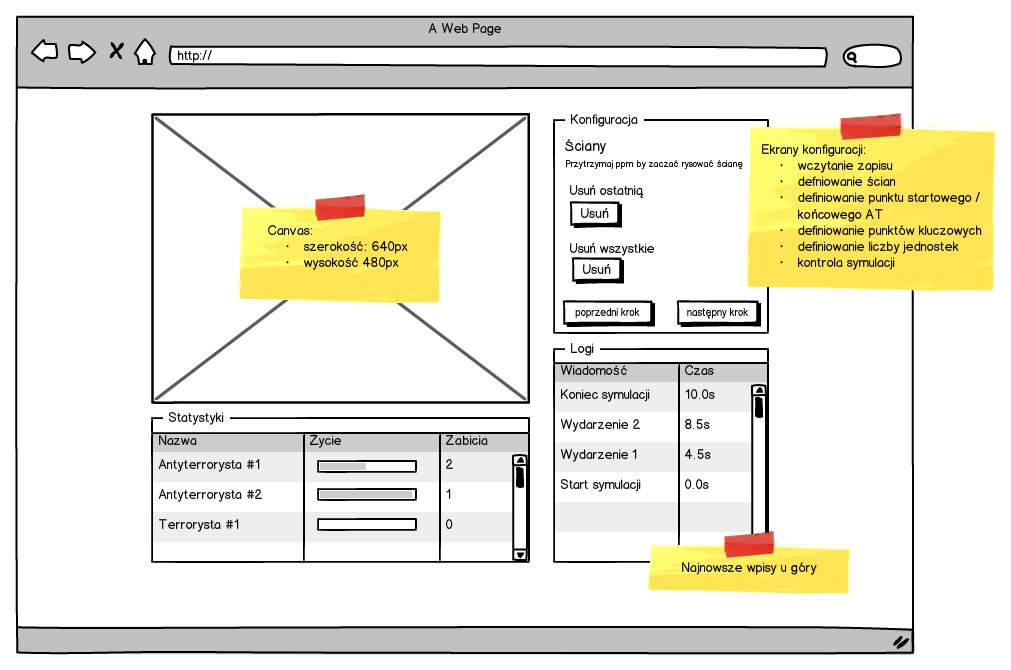
\includegraphics[width=160mm,height=106mm]{images/wireframe}
	\caption{Końcowy szkic interfejsu użytkownika\label{wireframe}}
\end{center}
\end{figure}

\section{Wymagania niefunkcjonalne}
Zestaw wymagań niefunkcjonalnych dla gry symulacyjnej, będącej przedmiotem tej pracy dyplomowej, został przedstawiony w tabeli \ref{nonFunc}. Po zaimplementowaniu aplikacji, została pozytywnie zweryfikowana zgodność z przywołanymi przeglądarkami\footnote{do weryfikacji została użyta usługa http://www.browserstack.com/}.

\begin{table}
\begin{center}
\begin{tabular}{|p{1.0\textwidth}|}
\hline
	\begin{itemize}
		\setlength\itemsep{0pt}		
		\item System operacyjny: Windows, Linux lub MacOS
		\item Przeglądarka internetowa: 
			\begin{itemize}
				\item Chrome w wersji 15.0 lub wyższej
				\item Firefox w wersji 4.0 lub wyższej
				\item Internet Explorer w wersji 9.0 lub wyższej
				\item Safari w wersji 5.1 lub wyższej
			\end{itemize} 
	\end{itemize}
\\\hline
\end{tabular}
\caption {Lista wymagań niefunkcjonalnych\label{nonFunc}}
\end{center}
\end{table} 

\section{Słownik pojęć}\label{dictonary}
Podczas sporządzania specyfikacji gry symulacyjnej, która jest przedmiotem tej pracy dyplomowej, niezbędne było dokładne zdefiniowanie niektórych wykorzystywanych pojęć. Poniżej znajduje się lista pojęć, uporządkowana alfabetycznie.

\begin{description}
	\item[Antyterrorysta] jest to jednostka, która w grze symulacyjnej oznaczona jest kolorem niebieskim. Celem antyterrorysty jest eliminacja wszystkich terrorystów
	\item[Antyterrorysta lider] jest to antyterrorysta, który prowadzi oddział antyterrorystyczny. Reszta antyterrorystów podąża za liderem. Liderem jest wybierana pierwsza żyjąca jednostka na liście antyterrorystów
	\item[Interfejs] jest to część aplikacji, która służy do przygotowania konfiguracji, sterowania symulacją oraz prezentacji logów i statystyk jednostek
	\item[Jednostka] jest to obiekt ruchomy, wykazujący pewne działanie taktyczne. W grze symulacyjnej jednostkami są terroryści i antyterroryści
	\item[Konfiguracja] są to dane o położeniu ścian, punktu startowego / końcowego antyterrorystów oraz punktów kluczowych. Konfiguracja może być zapisana, wczytana lub usunięta z poziomu interfejsu
	\item[Obiekt ruchomy] jest nim każda jednostka oraz każdy pocisk
	\item[Punkt kluczowy] jest to punkt należący do uporządkowanego zbioru, na podstawie którego budowane są ścieżki dla antyterrorystów. Wokół punktów kluczowych tworzeni są terroryści na początku rozgrywki
	\item[Punkt startowy / końcowy] jest to punkt, w którym są tworzeni i do którego wracają antyterroryści po przejściu przez wszystkie punkty kluczowe
	\item[Scena] jest to część interfejsu ukazująca mapę lokacji oraz ruchome obiekty
	\item[Statystyki] jest to część interfejsu ukazująca aktualny stan punktów życia oraz ilość zabić dla poszczególnych jednostek.
	\item[Symulacja] jest to stan gry, w którym na scenie znajdują się jakiekolwiek jednostki	
	\item[Terrorysta] jest to jednostka, która w grze symulacyjnej oznaczona jest kolorem czerwonym. Celem terrorysty jest obrona terytorium przed antyterrorystami
	\item[Warstwa sceny] jest to część sceny, do której aplikacja może przypisać obiekty w~celu późniejszego renderowania.
	\item[Zamknięcie konfliktu] jest to sytuacja, w której nie żyją wszyscy antyterroryści lub nie żyją wszyscy terroryści.
\end{description}


